\documentclass[aps,notitlepage]{revtex4-1}
\usepackage{color}
\usepackage{graphicx}
\usepackage{epstopdf}
\epstopdfsetup{update}
\usepackage{amsmath}
\usepackage{mathtools}
\usepackage[colorlinks,linkcolor=blue,anchorcolor=blue,citecolor=blue,urlcolor=blue]{hyperref}
\newcommand{\bea}{\begin{eqnarray}}
\newcommand{\eea}{\end{eqnarray}}
\newcommand{\bF}{\mathbf{F}}
\newcommand{\ba}{\mathbf{a}}
\newcommand{\bA}{\mathbf{A}}
\newcommand{\bu}{\mathbf{u}}
\newcommand{\bg}{\mathbf{g}}
\newcommand{\bB}{\mathbf{B}}
\newcommand{\bd}{\mathbf{d}}
\newcommand{\be}{\mathbf{e}}
%\newcommand{\bm}{\mathbf{m}}
\newcommand{\bM}{\mathbf{M}}
\newcommand{\bv}{\mathbf{v}}
\newcommand{\bV}{\mathbf{V}}
\newcommand{\bp}{\mathbf{p}}
\newcommand{\bq}{\mathbf{q}}
\newcommand{\bP}{\mathbf{P}}
\newcommand{\br}{\mathbf{r}}
\newcommand{\bx}{\mathbf{x}}
\newcommand{\bR}{\mathbf{R}}
\newcommand{\bN}{\mathbf{N}}
%\newcommand{\bell}{\boldsymbol{\ell}}
\newcommand{\bL}{\mathbf{L}}
\newcommand{\btau}{\boldsymbol{\tau}}
\newcommand{\bT}{\mathbf{T}}
\newcommand{\bi}{\mathbf{i}}
\newcommand{\bj}{\mathbf{j}}
\newcommand{\bk}{\mathbf{k}}
\newcommand{\bn}{\mathbf{n}}
\newcommand{\bomega}{\boldsymbol{\omega}}
\newcommand{\md}{\mathrm{d}}
\newcommand{\ie}{\textit{i.e.{ }}}
\newcommand{\etc}{\textit{etc.{ }}}
\newcommand{\ddt}{\frac{\md}{\md t}}
\newcommand{\ddtt}{\frac{\md^2}{\md t^2}}
\newcommand{\ppt}{\frac{\partial}{\partial t}}
\newcommand{\pptt}{\frac{\partial^2}{\partial t^2}}
\newcommand{\me}{\mathrm{e}}


%===============================================
\begin{document}
\title{Critical exponents of the nonlinear sigma model on Grassmann manifold $U(N)/U(m)U(N-m)$ by $1/N$ expansion}
\author{Da Wang}
\affiliation{Nanjing University}
\begin{abstract}
	Motivated by the numerical observation of the continuous phase transition between Neel and paramagnetic phases in the SU(N) Hubbbard model, we study its low energy nonlinear sigma model on Grassman manifold $U(N)/U(m)U(N-m)$ using the complex projective presentation, which is a generalization of the CP$^{N-1}$ model. Up to the first order of $1/N$, the critical exponents are obtained for space-time dimension $2<d<4$. Our results show that larger $m$ strongly suppresses the correlation length exponent $\nu$ and anomalous dimension $\eta$ as a result of stronger quantum fluctuation.
\end{abstract}
\maketitle



\section{from nonlinear sigma model to $U(N)/U(m)U(N-m)$ model}
Define complex projective representation \bea n_b=\sum_i z_i^\dag \sigma_b z_i=\mathrm{Tr}(Z^\dag\sigma_b Z) \eea  where $Z$ is a complex $N\times m$ matrix and $\sigma_b (b\le N^2-1)$ denote the generators of the $SU(N)$ group under the normalization $\mathrm{tr}(\sigma_b^2)=N$ in this work. ({\color{red}How about other choices?}) Then, using the relation (Fierz identity of the $SU(N)$ group) 
\bea (\sigma_b)_{\alpha\beta} (\sigma_b)_{\gamma\delta}+\delta_{\alpha\beta}\delta_{\gamma\delta}=N\delta_{\alpha\delta}\delta_{\beta\gamma} \eea
we get
\bea \bn\cdot\bn = N\mathrm{Tr}(ZZ^\dag Z Z^\dag)-\mathrm{Tr}(ZZ^\dag)^2 \eea
In order to maintain $\bn\cdot\bn=1$, we require a constraint condition \bea Z^\dag Z=\frac{1}{\sqrt{m(N-m)}}I \label{eq:normalizeZ}\eea
which tells the $Z$ fields live on the Grassmann manifold $U(N)/U(m)U(N-m)$. 

Now the nonlinear sigma model becomes
\bea S=\frac{\rho_s}{2}\int\partial_\mu\bn \cdot \partial_\mu\bn&=&\frac{\rho_s}{2}\int\partial_\mu \mathrm{Tr}(Z^\dagger\sigma_b Z) \partial_\mu \mathrm{Tr}(Z^\dagger \sigma_b Z) \nonumber\\
&=& N\rho_s \int\mathrm{Tr}\left[-(i\partial_\mu Z^\dagger Z) (-iZ^\dag \partial_\mu Z) + Z^\dag Z (i\partial_\mu Z^\dagger)(-i\partial_\mu Z)\right] \eea 
After Hubbard-Stratonovich transformation, we get
\bea S=N\rho_s\int \mathrm{Tr}\left[ (i\partial_\mu Z^\dag+A_\mu Z^\dag)(-i\partial_\mu Z+ZA_\mu)  \right] \eea
The constraint condition Eq.~\eqref{eq:normalizeZ} can be incorporated by a real Lagrangian multiplier matrix $\lambda$, which then brings us to
\bea \boxed{ S=N\rho_s\int \mathrm{Tr}\left[ (i\partial_\mu Z^\dag+A_\mu Z^\dag)(-i\partial_\mu Z+ZA_\mu)  \right] + i\int\mathrm{Tr}\left\{\lambda\left[Z^\dag Z-\frac{1}{\sqrt{m(N-m)}}I\right]\right\} } \eea
We can also rescale $Z$ field to another form
\bea \boxed{ S=\int \mathrm{Tr}\left[ (i\partial_\mu Z^\dag+A_\mu Z^\dag)(-i\partial_\mu Z+ZA_\mu)  \right] + i\int\mathrm{Tr}\left\{\lambda\left[Z^\dag Z-\frac{N\rho_s}{\sqrt{m(N-m)}}I\right]\right\} } \eea
{\color{red} I prefer to use the second form in the following since the propagators and vertices are as usual. We can also define a new parameter $g$ such that the constraint condition is $Z^\dag Z=(N/g)I$ or $(2N/g)I$ as in different literatures.} Notice the representation $n_b=\mathrm{Tr}(Z^\dag \sigma_b Z)$ has a gauge redundancy, \ie $Z\rightarrow ZU$ (with $U$ a $m\times m$ unitary matrix). Therefore, the gauge field is also non Abelian and can be parametrized as $A_\mu=f^aA_\mu^a$ [$f^a$ are adjoint representation of $SU(m)$ with $0\le a\le m^2-1$].


%Integrate over $Z$ and $Z^\dag$, we get
%\bea S_{\rm eff}=N\mathrm{Tr}\log(G^{-1})-i\frac{N\rho_s}{\sqrt{m(N-m)}}\mathrm{Tr}(\lambda) \label{eq:Seff}\eea
%where the prefactor $N$ in the first term comes from the sum of the SU(N) index. Now the $\mathrm{Tr}$ means summation over all remaining spaces: $d+1$-spacetime and m-dimensional subspace. The explicit expression of $G^{-1}$ is
%\bea G^{-1}(ki;k'j)&=&k^2\delta_{kk'}\delta_{ij}+k A_{ji}(k-k')+k' A_{ij}(k-k')+A_{\ell i}(p)A_{j \ell}(k-k'-p) \nonumber\\ &+& i\lambda_{ji}(k-k') \eea

\section{large-N limit: mean field approximation}
Suppose \bea Z_{\alpha i}=z_0\delta_{\alpha i}+z_{\alpha i}. \eea 
where $\alpha\le N$ and $i\le m$. $z_0\ne0$ means condensation occurs corresponding to the ordered state with \bea \sigma_b=\mathrm{diag}\left[\sqrt{\frac{N-m}{m}},\cdots,-\sqrt{\frac{m}{N-m}},\cdots\right]. \eea 

When $N=\infty$, the mean field approximation is expected to be exact as a result of the global prefactor $N$ after integrating out the $Z$-field. The saddle point condition gives 
\bea A_\mu=0 \eea which means no gauge field, and 
\bea z_0^2 + NT\int \frac{1}{k^2} = \frac{N\rho_s}{\sqrt{m(N-m)}} \eea
which is just the constraint condition.
The longitudinal magnetic susceptibility is
\bea \chi_{bb}(q)= m(N-m) z_0^4\delta_{q0} + (N-m)\frac{z_0^2}{q^2} + mNT\int \frac{1}{k^2(k+q)^2} \eea




\begin{itemize}
	\item $G(k)\sim k^{\eta-2}$ at $T=T_c$: $g(k)=k^{-2}$ gives $\eta_z=0$, while $\chi(q)\sim q^{d-4}$ gives $\eta_n=d-2$.
	\item $M\sim t^\beta$ (where $t=(T_c-T)/Tc$) below $T_c$: $M=\sqrt{m}z_0^2\sim t$ gives $\beta=1$.
  \item $\gamma$ can be obtained from $g^{-1}(k=0)$ (zero frequency) and $\nu$ can be obtained from $\xi$ (equal time correlation).
  \item In the conventional theory of critical phenomena, there is only one correlation length $\xi$, and thus all physical quantities share the same $\nu$. Such a situation may change, \textit{e.g.} in the deconfined quantum critical phenomena. What about tri-critical point?
\end{itemize}

\section{$1/N$-expansion}

\begin{figure}
	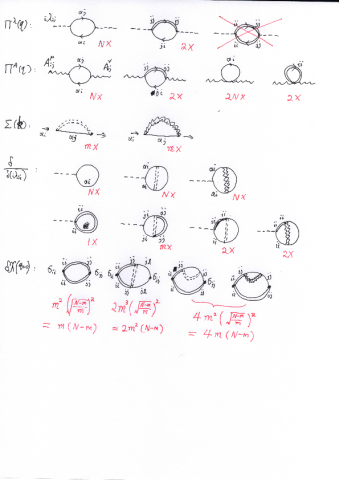
\includegraphics[width=0.6\textwidth]{1-N.png}
\end{figure}

In the order of $1/N$, the vacuum polarization of the $i\lambda$ field is
\bea \Pi_{ij}^\lambda(q)&=&2z_0^2\frac{1}{q^2} + NT\int \frac{1}{k^2(k+q)^2} = \Pi_\lambda(q) \eea
where \bea \Pi_\lambda(q)=\frac{2z_0^2}{q^2}+\frac{TNK_dA_d}{q^{4-d}} \eea 
There is also a $\delta_{q0}$ term with two condensation lines, but it can be safely removed when studying critical phenomena. ({\color{red} Any stronger argument?}) Then, we get the propagator of the $i\lambda$ field $D_\lambda(q)=-\Pi_\lambda^{-1}$. 
For the gauge field, the vacuum polarization under Landau gauge (for other gauge we need to add an additional divergence term in the Lagrangian) is
\bea \Pi_{ij}^{\mu\nu}(q) &=& NT\int \frac{(2k_\mu+q_\mu)(2k_\nu+q_\nu)}{k^2(k+q)^2} + 2z_0^2 \frac{q_\mu q_\nu}{q^2} - 2NT\int \frac{1}{k^2}\delta_{\mu\nu} - 2z_0^2 \delta_{\mu\nu} \nonumber\\ &=&\Pi_A(q)\left(\frac{q_\mu q_\nu}{q^2}-\delta_{\mu\nu}\right)\eea
where \bea \Pi_A(q)= 2z_0^2+\frac{TNK_dA_d}{d-1} q^{d-2} \eea
Then we get the gauge field propagator $D_A^{\mu\nu}(q)=-\Pi_A^{-1}\left(\frac{q_\mu q_\nu}{q^2}-\delta_{\mu\nu}\right)$. 

The self energy of the $z$ field is $\Sigma=\Sigma_\lambda+\Sigma_A$ where
\bea \Sigma_\lambda(k)=mT\int \left[\frac{1}{(k+q)^2}-\frac{1}{q^2}\right]D_\lambda(q)=-mT\int \left[\frac{1}{(k+q)^2}-\frac{1}{q^2}\right]\frac{1}{\Pi_\lambda} \eea
and
\bea \Sigma_A(k)=mT\int \frac{1}{(k+q)^2} D_A^{\mu\nu}(q) (2k_\mu+q_\mu) (2k_\nu+q_\nu) = 4mT\int \frac{1}{(k+q)^2}\frac{1}{\Pi_A}\left[ k^2-\frac{(k\cdot q)^2}{q^2} \right] \eea 
from the $k^2\ln k$ term, we immediately get $\eta_z=-\frac{(4d-7)m}{NA_d}$. [Hikami(1980)]

The constraint condition is now
\bea NT\int \frac{1}{k^2} + NT\int \frac{1}{k^4}\Sigma(k) + z_0^2 \left[ 1-  mT\int \frac{1}{k^4} \frac{1}{\Pi_\lambda} + 2 \left.\frac{\Sigma(k)}{k^2}\right|_{k\rightarrow0}\right] = \frac{N\rho_s}{\sqrt{m(N-m)}} \eea 

The susceptibility is 
\bea m(N-m)z_0^4\delta_{q0}\left[  1-  2mT\int \frac{1}{k^4} \frac{1}{\Pi_\lambda} + 4 \left.\frac{\Sigma(k)}{k^2}\right|_{k\rightarrow0} \right] \eea

Then following IKK(1996), the critical exponent $\beta$ can be easily obtained
\bea \beta=1-Q=1-\frac{2m(d^2-d+2)}{NA_d} \eea 

The exponent $\nu$ can be obtained from $\eta_z$ and $\gamma_z$ following HLM(1974), Hikami(1980) or KS(2008). (check it?) The result is [Hikami(1980)]
\bea \nu=\frac{1}{d-2}\left[ 1-\frac{2md(d-1)}{NA_d} \right] \eea

From $\beta$ and $\nu$, all remaining exponents can be obtained.
\bea \gamma_n=\frac{4-d}{d-2}\left[ 1+\frac{8m(d-2)}{(4-d)NA_d}-\frac{2md(d-1)}{NA_d} \right] \eea
\bea \eta_n=(d-2)\left[1-\frac{8m}{NA_d}\right] \eea


{\color{red} The bad news is: we should take $m/N$ as a small parameter to valid the $1/N$-expansion calculation. Therefore, the method cannot be applied to our interested case with $m=N/2$. Anyway, let us keep going on and just take this work as a generalization of the $m=1$ theory.}

\begin{appendix}
	
\section{Irkhin, Katanin, and Katsnelson (1996)}
Up to logarithmic accuracy, the z-field self energy is [Eq.17 in IKK(1996)]
\bea \Sigma=\Sigma_A-\Sigma_\lambda\sim\frac{4d-7}{d-2}\frac{k^2}{NA_d}\ln\left(\frac{\Lambda^{d-2}}{\mathrm{max}(k^{d-2},n_B)}\right) \eea
The logarithmic divergence gives \bea \eta_z=-\frac{4d-7}{NA_d} \eea in agreement with Halperin, Lubensky and Ma (1974) at $d=3$.

The following three terms/integrals are in need
\bea &&\left.\frac{\Sigma}{k^2}\right|_{k\rightarrow0}=\frac{4d-7}{d-2}\frac{1}{NA_d}\ln\left(\frac{\Lambda^{d-2}}{n_B}\right) \sim -\frac{4d-7}{d-2}\frac{1}{NA_d}\ln n_B \\
&&\frac{T}{N}\int \frac{1}{k^4\Pi_\lambda(k)} \sim -\frac{1}{(d-2)NA_d}\ln n_B \\
&&\int \frac{\Sigma(n_B)-\Sigma(n_B=0)}{k^4} \sim \frac{2(d^2-d+2)}{NA_d} n_B \ln n_B \eea 

The constraint equation [Eq.16 in IKK(1996)] is
\bea 1=\frac{gT}{2}\int\frac{1}{k^2}+\frac{gT}{2}\int\frac{\Sigma}{k^4} + n_B\left(1-\frac{T}{N}\int \frac{1}{k^4\Pi_\lambda} + 2\left.\frac{\Sigma}{k^2}\right|_{k\rightarrow0} \right) \eea

Set $n_B=0$ we get $T_c$
\bea \frac{2}{gT_c}=\int \frac{1}{k^2} + \int \frac{\Sigma(n_B=0)}{k^4} \eea
and when $n_B\ne0$ we have
\bea \frac{2}{gT}=\int \frac{1}{k^2}+\int \frac{\Sigma(n_B)}{k^4} + \frac{2n_B}{gT} \left(1-\frac{T}{N}\int \frac{1}{k^4\Pi_\lambda} + 2\left.\frac{\Sigma}{k^2}\right|_{k\rightarrow0} \right) \eea
from the above two equations, we get (up to logarithmic accuracy)
\bea t\propto\frac{2}{gT}-\frac{2}{gT_c}=\frac{2n_B}{gT_c}\left(1+(Q-P)\ln n_B\right)\sim n_B^{1+Q-P} \eea 
where
\bea P=\frac{8d-15}{(d-2)NA_d} \quad \text{and} \quad Q=\frac{2(d^2-d+2)}{NA_d} \eea 

The order parameter can be obtained from zero momentum susceptibility [Eq.18 in IKK(1996)]
\bea m^2\propto\delta\chi&=&\delta_{q0}\frac{n_B^2}{2N}\left( 1-\frac{2T}{N}\int \frac{1}{k^4\Pi_\lambda} + 4\left.\frac{\Sigma}{k^2}\right|_{k\rightarrow0} \right) \\
&=&\delta_{q0}\frac{n_B^2}{2N}\left(1-2P\ln n_B\right) \\
&\sim&\delta_{q0}\frac{n_B^{2-2P}}{2N}\propto t^{2(1-P)(1-Q+P)}\delta_{q0}=t^{2(1-Q)}\delta_{q0} \eea
Then, from the definition of $\beta$, \ie $m\propto t^{\beta}$, we get
\bea \beta=1-Q=1-\frac{2(d^2-d+2)}{NA_d} \eea 




\section{bubble integrals \& logarithmic divergence}
Using the trick of Feynman parameter (see Peskin's book, Ch6.3)
\bea \frac{1}{AB}=\int_0^1 \md \alpha \frac{1}{[\alpha A+(1-\alpha)B]^2} \eea
the bubble integrals can be completed (Irkhin {\it et al.}, 1996)

\bea \int \frac{1}{k^2(k+q)^2} = \frac{K_d A_d}{q^{4-d}} \eea
where 
\bea K_d^{-1}=2^{d-1}\pi^{d/2}\Gamma\left(\frac{d}{2}\right) \eea
\bea A_d=\frac{\Gamma(d-2)\Gamma(2-d/2)\Gamma^2(d/2-1)}{2\Gamma(d-2)} \eea



The above bubble integral can be completed using Feynman parameters together with the following relations:
\bea \int_0^\infty \frac{x^{\alpha-1}}{(1+x)^{\alpha+\beta}}\md x=B(\alpha,\beta)=\frac{\Gamma(\alpha)\Gamma(\beta)}{\Gamma(\alpha+\beta)} \eea 
\bea \int_0^1 t^{x-1}(1-t)^{y-1}dt = B(x,y) \eea 
\bea \int_0^{\pi/2} \sin^{2\alpha-1}(\theta)\cos^{2\beta-1}(\theta)\md \theta=\frac{B(\alpha,\beta)}{2} \eea
from which we get a useful relation $\langle \cos^2\theta \rangle=1/d$. 


\bea \int \frac{\md^d\bq}{(2\pi)^d} q^{4-d}\left[ \frac{1}{(\bk+\bq)^2}-\frac{1}{q^2} \right]
&=& k^2\int^{1/k}\frac{-2q\cos\theta-1}{q^2(q^2+2q\cos\theta+1)}q^{4-d} q^{d-1}\md q \frac{S_{d-1}}{(2\pi)^d} \sin^{d-2}\theta \md\theta \eea
Notice that the logarithmic divergence comes from large $q$ and thus we keep only large $q$ terms
\bea \int = k^2\frac{S_{d-1}}{(2\pi)^d} \int \frac{4\cos^2\theta-1}{q^4}q^{4-d}q^{d-1}\md q \sin^{d-2}\theta \md \theta \eea
Since $\langle \cos^2\theta\rangle=1/d$, we have
\bea \int = K_d k^2\left(\frac{4}{d}-1\right)\ln k \eea 


Let's attack the following integral:
\bea \int \frac{\Sigma_A-\Sigma_\lambda}{k^4} \eea 

In order to complete the awesome task, we first need three bubble integrals:
\bea \int_k \frac{1}{k^2(k+q)^2} = \frac{K_d}{2} B\left( \frac{d}{2}-1,\frac{d}{2}-1 \right) B\left( \frac{d}{2},2-\frac{d}{2} \right) q^{d-4} = K_d A_d q^{d-4}\eea
\bea \int_k \frac{k\cdot q}{k^4(k+q)^2}=-K_d B\left(\frac{d}{2},3-\frac{d}{2}\right)B\left(\frac{d}{2}-1,\frac{d}{2}-1\right) q^{d-4} = -\left(2-\frac{d}{2}\right) K_d A_d q^{d-4} \eea
\bea \int_k \frac{(k\cdot q)^2}{k^4(k+q)^2} = K_d B\left(\frac{d}{2}-1,\frac{d}{2}\right)\left[\frac{1}{d}B\left(\frac{d}{2}+1,2-\frac{d}{2}\right)+B\left(\frac{d}{2},3-\frac{d}{2}\right)\right] q^{d-2} = \frac{5-d}{4} K_dA_d q^{d-2}\eea 

Using the above three bubble integrals, we have
\bea \int \frac{\Sigma_A}{k^4} = (d-1) \frac{TK_dA_d}{N} \int_q \frac{1}{q^{4-d}\Pi_A} \eea

\bea \int \frac{\Sigma_\lambda}{k^4} = (3-d) \frac{TK_dA_d}{N} \int_q \frac{1}{q^{6-d}\Pi_\lambda} \eea

Then Let's examine q-integrals
\bea \int \frac{1}{q^{4-d}\Pi_A}=\frac{d-1}{TA_d}\int \frac{q^{2d-5}\md q}{q^{d-2}+\frac{4(d-1)n_B}{gTK_dA_d}} \sim \frac{d-1}{TA_d}\frac{1}{d-2}\frac{4(d-1)}{gTA_dK_d} n_B \ln n_B \eea
and 
\bea \int \frac{1}{q^{6-d}\Pi_\lambda}=\frac{1}{TA_d} \int \frac{q^{2d-5}\md q}{q^{d-2}+\frac{4n_B}{gTK_dA_d}} \sim \frac{1}{TA_d}\frac{1}{d-2}\frac{4}{gTK_dA_d} n_B \ln n_B \eea
Combining the above two expressions, we have
\bea \frac{gT}{2}\int \frac{\Sigma_A-\Sigma_\lambda}{k^4} \sim \frac{2(d^2-d+2)}{NA_d} n_B\ln n_B \eea 

\section{spherically symmetric integrals in general dimensions}
Following Goldenfeld's book
\bea \int \frac{\md^d\bq}{(2\pi)^d}=\frac{S_d}{(2\pi)^d}\int q^{d-1}\md q = \frac{S_{d-1}}{(2\pi)^d}\int q^{d-1}\sin^{d-2}\theta \md q \md \theta \eea
where \bea S_d=\frac{2\pi^{d/2}}{\Gamma(d/2)} \eea



\section{next?}
\begin{itemize}
\item How to get reasonable critical exponents for fixed $m/N\sim1/2$? 
\item A RG study? $\varepsilon$-expansion?
\item If the phase transition is a deconfined one, how to include the effect of topological terms?
\item See Kaul and Sachdev, 2008. A study on fermion-boson mixed model? supersymmetry?
\item See recent researches on fermion-induced QCP, {\it e.g.} Hong Yao, Herbut.
\end{itemize}

\end{appendix}


\begin{references}
\bibitem{} Shang-Keng Ma, 1973 (very well written); Shang-Keng Ma, Modern theory of critical phenoma, \S9.4. (only real field)
\bibitem{} Zinn-Justin, quantum field theory and critical phenomena.
\bibitem{} Auerbach, Interacting electrons and quantum magnetism, \S14.1.
\bibitem{} Halperin, Lubensky and Ma, 1974; Nogueira and Kleinert, Field theoretical approaches to the superconducting phase transition, 2003. Solve $\eta_z$ and $\nu_z$ (assuming equal to $\nu_{Neel}$) from single particle Green's function.
\bibitem{} Macfarlane, 1977; Duerksen, 1981; Maharana, 1983. (about $U(N)/U(m)U(N-m)$ model)
\bibitem{} Hikami, 1980. (closely related but only single particle exponents obtained)
\bibitem{} Arovas and Auerbach, 1988.
\bibitem{} Read and Sachdev, 1989; 1990. (relation with Young tableau)
\bibitem{} Irkhin, Katanin and Katsnelson, 1996. Solve $\beta_{Neel}$ and $\nu_{Neel}$ directly from spin-spin Green's function.
\bibitem{} Takashima, 2006
\bibitem{} Kaul and Sachdev, 2008. Solve $\eta_{Neel}$ from $\eta_z$ and vertex correction (seems easier)
\bibitem{} Saito et al., 2012. Solve $\nu$ from 2PI? [exponent $\mu$ defined in Ma(1973)]
\end{references}
%\bibliography{all}
\end{document}
